\chapter{Model} \label{chap:two}

% Parameter Table
\begin{table}
	\rowcolors{1}{}{lightgray}
	\centering
	\caption{Model parameters. \label{table:parameters}}
	\begin{tabular}{c p{.25in} p{4.5in}}
		$m$ & & Number of fibers \\
		$n_j$ & & Number of particles on fiber $j$, $1 \leq j \leq m$ \\
		$n_+$ & & Number of particles on the top substrate \\
		$n_-$ & & Number of particles on the bottom substrate \\
		$\delta_j$ & & Attachment point for fiber $j$ on bottom substrate, $1 \leq j \leq m$ \\
		$\ell$ & & Equilibrium distance for extensible springs \\
		$\ell_+$ & & Spacing between particles on the top substrate \\
		$\ell_-$ & & Spacing between particles on the bottom substrate \\
		$\beta$ & & Strength of torsional springs \\
		$\gamma$ & & Spring constant for extensible springs \\
		$\varepsilon$ & & Strength of vdW force between particles of fibers \\
		$\varepsilon_+$ & & Strength of vdW force between a particle on a fiber and a particle on the top substrate \\
		$\varepsilon_-$ & & Strength of vdW force between a particle on a fiber and a particle on the bottom substrate \\
		$\sigma$ & & Equilibrium distance between two particles for vdW \\
		$(\mu,\lambda)$ & & Load applied to the moving substrate \\
		$(x^{(+)}_0,y^{(+)}_0)$ & & Initial position for first particle on the top substrate \\
		$(x^{(-)}_0,y^{(-)}_0)$ & & Initial position for first particle on the bottom substrate
	\end{tabular}
\end{table}
	
	\begin{figure}
		\begin{center}
			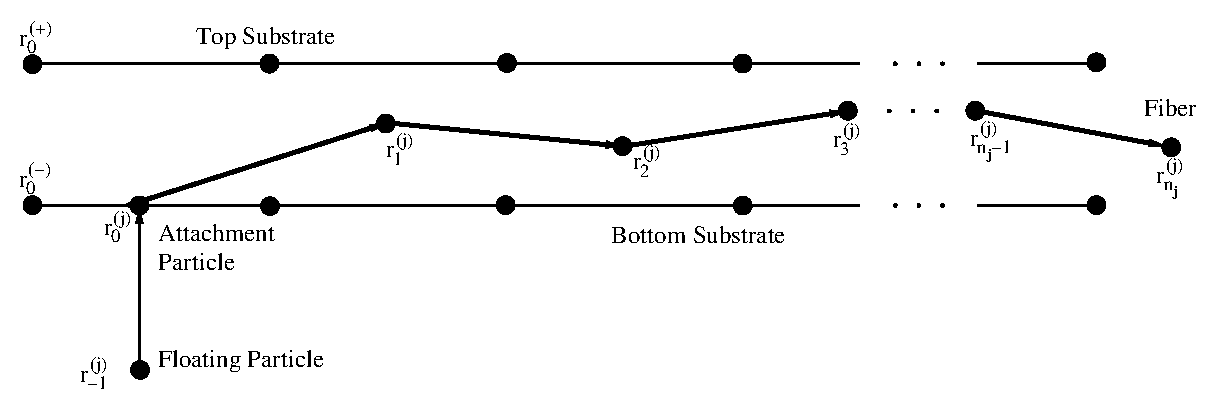
\includegraphics[scale=.75]{./old_fig/Geometry.eps}
		\end{center}		
		\caption{Geometry of a fiber pinned between the top and bottom substrates.
		\label{fig:Geometry}}
	\end{figure}		
	
\section{Geometry}

	We consider a collection of particles linked into a chain that we call a fiber. Each fiber is connected to a stationary horizontal (bottom) substrate at some fixed position. There are two artificial particles associated with each fiber, one being the attachment point with the substrate and an additional particle placed at any point on a half circle below the stationary substrate of radius one. We will call the attachment point the attachment particle, and the other particle below it the floating particle (see Fig.~\ref{fig:Geometry}).
	
We denote the position vector of the $i$th particle on the $j$th fiber by
\begin{equation}
	\textbf{r}_i^{(j)} = (x_i^{(j)},y_i^{(j)})
\end{equation}
where $1 \leq j \leq m$ and $1 \leq i \leq n_j$. We also define the following vectors,

\begin{equation}
	\Delta \textbf{r}_i^{(j)} = \textbf{r}_i^{(j)} - \textbf{r}_{i-1}^{(j)}.
\end{equation}
The two artificial particles are denoted as follows,
\begin{equation}
	\textbf{r}_0^{(j)} = (x_0^{(j)},y_0^{(j)}) = (\delta_j,0)
\end{equation}
for the attachment particle and
\begin{equation}
	\textbf{r}_{-1}^{(j)} = (x_{-1}^{(j)},y_{-1}^{(j)}).
\end{equation}
for the floating particle.

	In any given configuration there could be several fibers, each consisting of a contiguous chain of linked particles. Each particle can be thought of as a discretization of a neighborhood of bonded carbon atoms. Indeed, a chain of particles is intended to describe a CNT via a coarse-grained approach. This approach is sufficiently generic to describe other fiber structures.
	
	In addition to the $m$ fibers in the model are two horizontal substrates, both a top and bottom one. The bottom substrate as described before is attached to every fiber at the attachment particle. We define two sets position vectors,
\begin{eqnarray}
	\textbf{r}_0^{(+)} = (x_0^{(+)},y_0^{(+)}) \\
	\textbf{r}_i^{(+)} = (x_0^{(+)} + i\ell^+,y_0^{(+)})
\end{eqnarray}
for the top substrate and,
\begin{eqnarray}
	\textbf{r}_0^{(-)} = (x_0^{(-)},y_0^{(-)}) \\
	\textbf{r}_i^{(+)} = (x_0^{(+)} + i\ell^-,y_0^{(+)})
\end{eqnarray} 
for the bottom substrate. Both substrates have one predetermined particle, the $0th$ particle. The top substrate is allowed to move under a translational load but the bottom substrate is stationary (see Fig.~\ref{fig:Geometry}).

\section{Energy}

	An isolated fiber is in equilibrium when all particles on a chain are collinear and each particle is a fixed distance $\ell$ away from its neighbors. In order to achieve this equilibria configuration we incorporate two types of springs into the model: an extensible spring and a torsional spring.

\subsection{Extensible spring}

	The extensible spring is described by the standard Hooke's law and is meant to keep any two adjacent particles on a fiber a fixed distance $\ell$ apart. This can also be thought of as maintaining a length of $\ell$ for all links between particles. The energy for all springs is,
\begin{equation}
	E_e = \gamma \sum_{j=1}^m \sum_{i=1}^{n_j} \left[ \left( \|\Delta \textbf{r}_i^{(j)} \| - \ell \right)^2 \right].
\end{equation}
Note that, with our notation for a given fiber $j$ ,the sum starts with the first particle and the attachment particle of that fiber. The sum continues until the final particle on the fiber; it only has one adjacent neighbor.

	\begin{figure}
		\begin{center}
			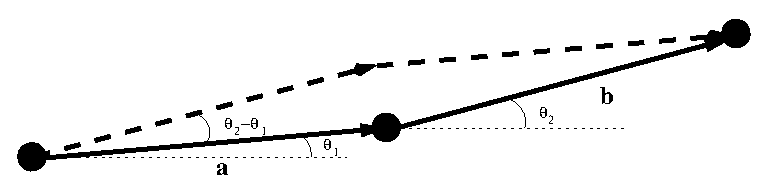
\includegraphics[scale=1]{./old_fig/BendingEnergy.eps}
		\end{center}		
		\caption{Two vectors $\textbf{a}$ and $\textbf{b}$, representing links between three particles and a corresponding angle measured against the positive $x$-axis centered at each tail point. The bending energy will be minimized when the difference in angle is zero, or the particles are collinear.
		\label{fig:BendingEnergy}}
	\end{figure}	

\subsection{Torsional spring}

	For a every fiber we want the energy to be minimized when the particles are collinear. To accomplish this we introduce the energy penalty for bending when the angle between adjacent links is not zero (see Fig.~\ref{fig:BendingEnergy}). A quadratic energy is not sufficient here because we expect that the energy should blow up when the links point in opposite directions. Therefore, we set 
\begin{equation}
	e_b = 2 \tan^2 \left( \frac{\Delta \theta}{2} \right),
\end{equation}
where $e_b$ is the energy of one junction between two links since the geometry is described in terms of particles and, not angles, we use double angle identities the definition of dot product to obtain the following expression for total bending energy for every fiber,
\begin{equation}
	E_b = 2\beta \sum_{j=1}^m \sum_{i=1}^{n_j} \left[ \frac{\|\Delta \textbf{r}_i^{(j)} \| \|\Delta \textbf{r}_{i-1}^{(j)} \| - \Delta \textbf{r}_i^{(j)} \cdot \Delta \textbf{r}_{i-1}^{(j)}}{\|\Delta \textbf{r}_i^{(j)} \| \|\Delta \textbf{r}_{i-1}^{(j)} \| + \Delta \textbf{r}_i^{(j)} \cdot \Delta \textbf{r}_{i-1}^{(j)}} \right].
\end{equation}

	This energy incorporates every contiguous set of three particles, including the two artificial particles. With the incorporation of the angle between the artificial particles and the first particle, the minimizing angle of the fiber with respect to the substrate can be tuned according to the placement of the floating particle. For example, if the angle between the floating particle and the attachment particle is $\frac{\pi}{2}$, then the entire fiber will want to be upright, if it is $\frac{\pi}{4}$, then the entire fiber will want be slanted at a $45^{\circ}$ angle, etc.

\subsection{van der Waals interactions}	

	\begin{figure*}[t!]
		\centering
		\begin{subfigure}[t]{.5\textwidth}
			\centering
			\includegraphics[scale=.5]{./fig/ch2/lj_e.eps}
			\caption{Lennard-Jones energy, well depth is $\varepsilon$, minimized at $\sigma$. \label{subfig:LJEnergy}}
		\end{subfigure}%
		~
		\begin{subfigure}[t]{.5\textwidth}
			\centering
			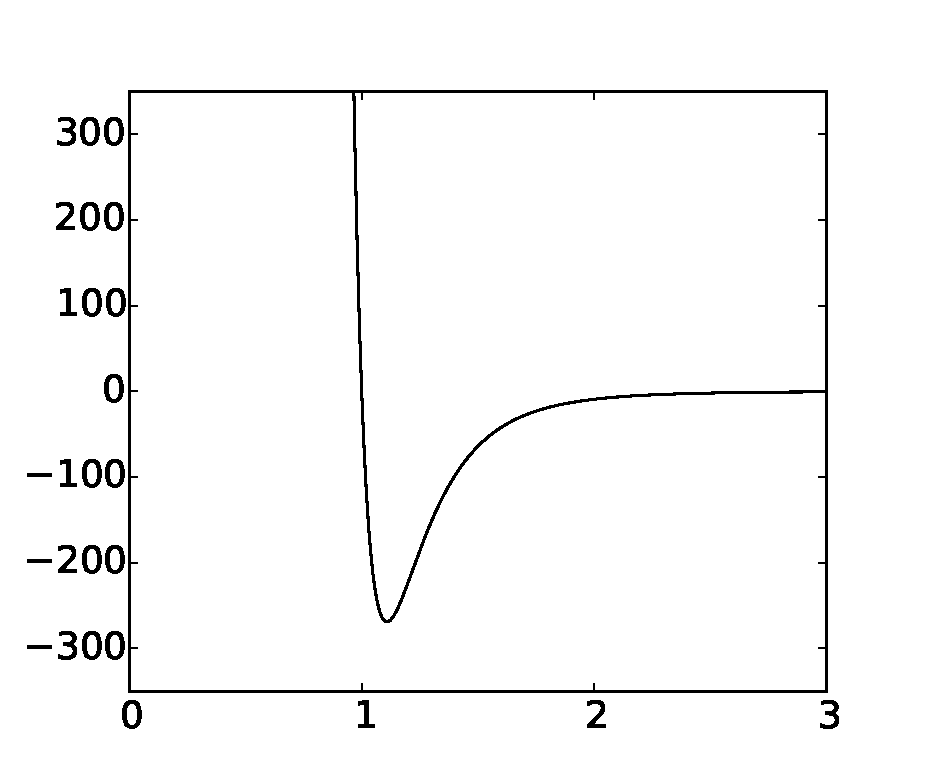
\includegraphics[scale=.5]{./fig/ch2/lj_f.eps}
			\caption{Lennard-Jones force. \label{subfig:LJForce}}
		\end{subfigure}		
		\caption{Lennard-Jones 12-6 potential and force with $\sigma = 1$ and $\varepsilon = 100$.\label{fig:LJ}}	
	\end{figure*}

	At a mesoscopic scale there is typically an interaction between a given particle and every other particle in the system, with $\mathcal{O}(n^2)$ interactions overall Here we use a truncated Lennard-Jones 12-6 potential to represent the van der Waals interactions between each particle in the model. However, because we already have a spring connecting adjacent particles, we don't incorporate an additional interaction between linked particles.
	
The standard Lennard-Jones potential,
\begin{equation}
	U(x) = \varepsilon \left[ \left( \frac{\sigma}{x} \right)^{12} - 2 \left( \frac{\sigma}{x} \right)^6 \right],
\end{equation}

	\begin{figure*}[t!]
		\centering
		\begin{subfigure}[t]{.5\textwidth}
			\centering
			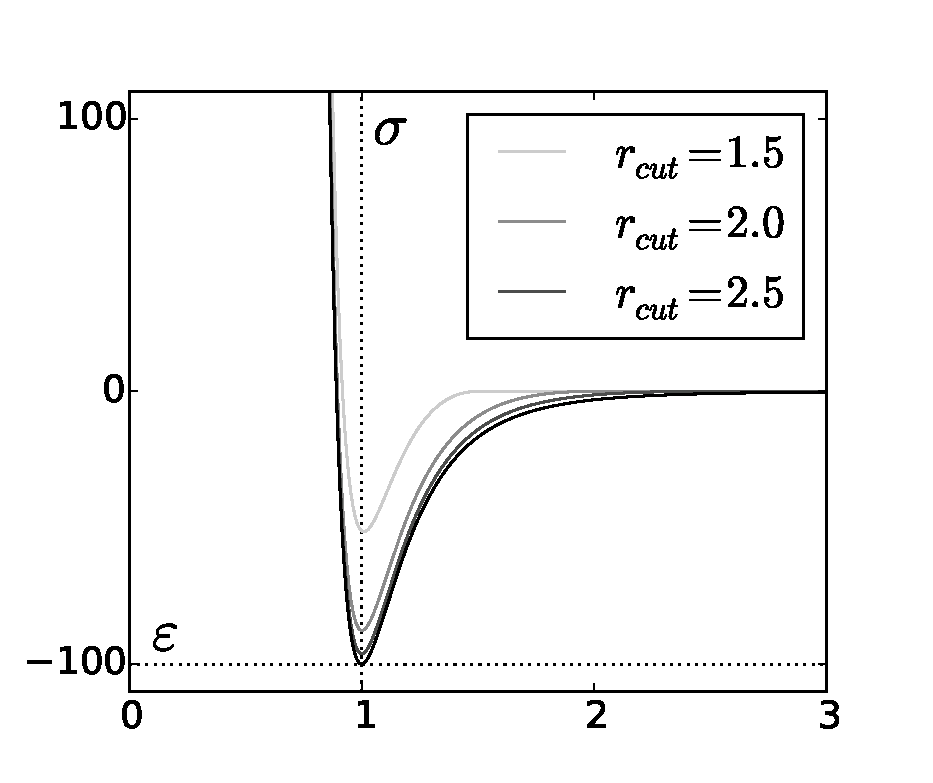
\includegraphics[scale=.5]{./fig/ch2/ljc_e.eps}
			\caption{Truncated Lennard-Jones energy. \label{subfig:LJTEnergy}}
		\end{subfigure}%
		~
		\begin{subfigure}[t]{.5\textwidth}
			\centering
			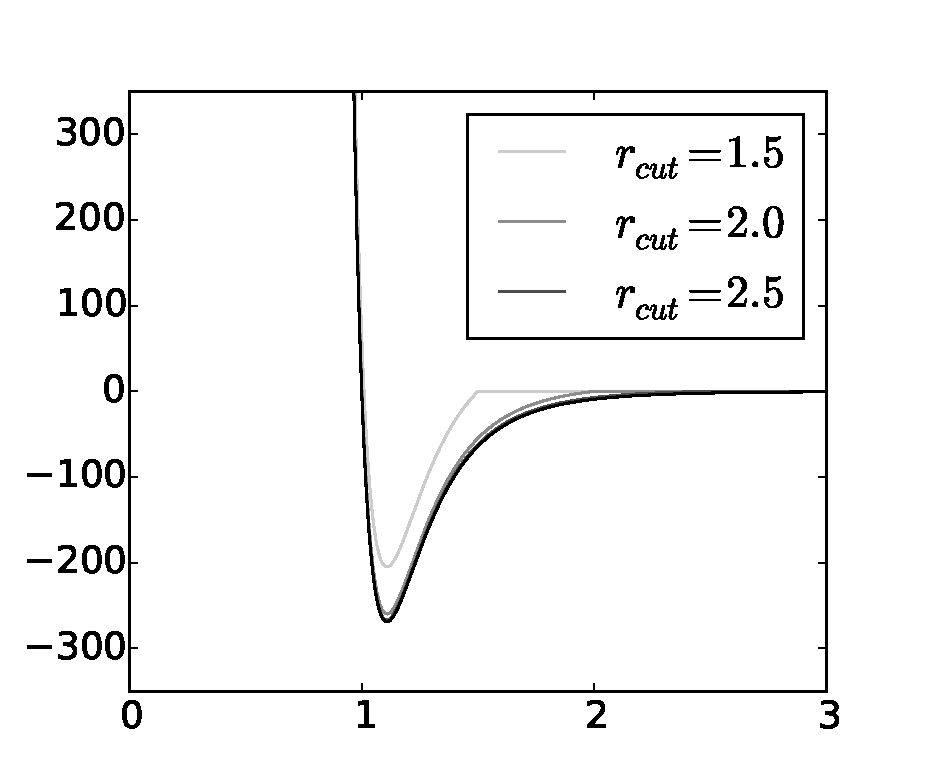
\includegraphics[scale=.5]{./fig/ch2/ljc_f.eps}
			\caption{Truncated Lennard-Jones force. \label{subfig:LJTForce}}
		\end{subfigure}		
		\caption{TODO(new plot with dashed lines and an internal legend) Truncated Lennard-Jones potential with $r_c = 1.5$ in red, $r_c = 2$ in green, $r_c = 3$ in blue, and the Lennard-Jones potential without cut in black.\label{fig:LJT}}	
	\end{figure*}	

\noindent	
asymptotically approaches zero as $x$ approaches infinity. This makes Lennard-Jones a short range potential and, more importantly, makes interactions at long distances negligible. We can then truncate (or cut) the potential at some radius $r_c$. However, this introduces a discontinuity in the potential, so in order to repair both the potential and it's derivative, we use the following modification.
\begin{equation}
	U_c(x) = \left\{ 
		\begin{array}{lr}
			U(x) - U(r_c) - \frac{dU}{dx}\bigg|_{x = r_c}(x - r_c), & x \leq r_c\\
			0, & x > r_c
		\end{array}
		\right. 
\end{equation}

	Clearly the sequence of truncated Lennard-Jones potentials converges to the Lennard-Jones potential as $r_c \to \infty$ and the truncated Lennard-Jones potentials share the same asymptotic behavior (see Fig.~\ref{fig:LJT}). This truncation technique is referred to as a shifted forces, it is commonly used to conserve energy in the potential and avoid potential artifacts with a model. The discontinuous truncation is more commonly used but can cause larger discrepancies in energy particularly with very long simulations. Although this method alters the potential everywhere the accuracy with respect to the true potential is still good, and in specific molecular dynamics simulations it has been observed as better than our alternative \cite{Toxvaerd2011}.
	
	For our model the potential is safer but likely unneeded due to our liberal cutoff selection of $r_c = 8$ in all simulations. However we are searching for equilibrium which can cause very long time intervals over the entire simulation, so to avoid artifacts in the geometry we use this variation of the truncated Lennard-Jones potential.

	In order to represent concisely the set of particles that a given particle is interacting with, we define the set
\begin{equation}
	P(j,i) = \{ (h,k)|j \neq h \vee k \neq i \pm 1, 1 \leq h \leq m, 1 \leq k \leq n_h \},
\end{equation}
which contains every particle that the $i$th particle on the $j$th fiber will be interacting with via the 12-6 potential. We now have the van der Waals energy for all pairs:
\begin{multline}
	E_v = \sum_{j=1}^m \sum_{i=1}^{n_j} \bigg[ \sum_{(h,k) \in P(j,i)} U_c \left( \| \textbf{r}_i^{(j)} - \textbf{r}_k^{(h)} \| \right) \\ + \sum_{k=1}^{n_-} U_c \left( \| \textbf{r}_i^{(j)} - \textbf{r}_k^{(-)} \| \right) + \sum_{k=1}^{n_+} U_c \left( \| \textbf{r}_i^{(j)} - \textbf{r}_k^{(+)} \| \right) \bigg],
\end{multline}
It is not necessarily the case that the interaction strength, $\varepsilon$, is the same for each potential. There are different strengths for fiber to fiber, fiber to top substrate, fiber to bottom substrate interactions respectively.

% van der Waals lower substrate pressure
%\begin{equation}
%	E_p = \sum_{j=1}^m \sum_{i=1}^{n_j} U_p \left( y_i^{(j)} \right)
%\end{equation}

\subsection{Total energy}

To complete the governing equation for the energy we also incorporate a vector load on the top substrate. In particular we apply a translational load to the point $(x_0^{(+)},y_0^{(+)})$. Adding up all contributions gives the total energy, 

% Total energy
\begin{equation}
	E = E_b + E_e + E_v + \lambda x_0^{(+)} - \mu y_0^{(+)}.
\end{equation}

\section{Dynamics}

Using Newton's second law with a damping term we have,

\begin{equation}
	M\frac{d^2\textbf{r}_i^{(j)}}{dt^2} + \frac{d\textbf{r}_i^{(j)}}{dt} = -\nabla_{\textbf{r}_i^{(j)}}E,
\end{equation}

	for some particle, where $M$ is the mass of that particle. We then assume the mass of particles we want to take into consideration is small enough to make the acceleration negligible, which leaves us with,
	
\begin{equation}
	 \frac{d\textbf{r}_i^{(j)}}{dt} = -\nabla_{\textbf{r}_i^{(j)}}E.
\end{equation}

Clearly in solving this ordinary differential equation we are minimizing the total energy of our system. Our first consideration then is to discuss minimizing equilibria of the total energy and second to discuss any dynamical considerations.

TODO(expand)

\section{Implementation}

	The model was first implemented using MATLAB \cite{MATLAB2010}, and then later translated into C using SUNDIALS\cite{sundials}. A Verlet neighbor list is used and dynamically updated at every time step when the sum in the two largest changes in position is greater than the buffer distance in the Verlet list (a static value of 4 in all simulations presented here). A simulation is considered in equilibrium when the max norm of the difference between the latest two solution vectors is less than a prescribed tolerance, and the difference between the latest two top substrate positions is less than the same tolerance. The system is also considered in equilibrium if the velocity of the top substrate is within the same tolerance of it's maximum velocity. Either of these conditions must be satisfied for ten time steps. The equilibrium tolerance is a static value, $10^{-8}$. Matplotlib was also used for several figures presented in this thesis \cite{Hunter2007}.







